\documentclass{article}
	
\usepackage[margin=1in]{geometry}		% For setting margins
\usepackage{amsmath}				% For Math
\usepackage[]{amssymb}
\usepackage{amsmath}
\usepackage{gensymb}
\usepackage{fancyhdr}				% For fancy header/footer
\usepackage{graphicx}				% For including figure/image
\usepackage{cancel}					% To use the slash to cancel out stuff in work
\usepackage{wasysym}                % For cent symbol
\usepackage{needspace}              % To force item to next page

%%%%%%%%%%%%%%%%%%%%%%
% Set up fancy header/footer
\pagestyle{fancy}
\fancyhead[RO,R]{{\large\textbf{PHYS-102}}}
\fancyhead[LO,L]{\large{\textbf{Ch 20 Problem Set}}}
% \fancyhead[CO,C]{\large{\textbf{Part 1}}}
% \fancyhead[RO,R]{\today}
\fancyfoot[LO,L]{}
\fancyfoot[CO,C]{\thepage}
\fancyfoot[RO,R]{}
\renewcommand{\headrulewidth}{0.4pt}
\renewcommand{\footrulewidth}{0.4pt}
%%%%%%%%%%%%%%%%%%%%%%

\newcommand{\hmwkTitle}{Ch 20 Second Law of Thermodynamics}
% \newcommand{\hmwkDueDate}{February 12, 2014}
\newcommand{\hmwkClass}{PHYS-102}
% \newcommand{\hmwkClassTime}{}
% \newcommand{\hmwkClassInstructor}{Professor Isaac Newton}
\newcommand{\hmwkAuthorName}{\textbf{\underline{\hspace{3in}}}}

% math shortcuts
\newcommand\rr{\quad\Rightarrow\quad}

%
% Title Page
%

\title{
    \vspace{2in}
    \textmd{\textbf{\hmwkTitle}}\\
    \vspace{0.5in}
    \textmd{\textbf{\hmwkClass}}\\
    % \normalsize\vspace{0.1in}\small{Due\ on\ \hmwkDueDate\ at 3:10pm}\\
    % \vspace{0.1in}\large{\textit{\hmwkClassInstructor\ \hmwkClassTime}}
    \vspace{4in}
}

\author{\hmwkAuthorName}
\date{}
\begin{document}
\maketitle
\newpage
\begin{center}
    \section*{\textbf{\underline {Conceptual Questions}}}
\end{center}
\subsubsection*{
    2. Can you warm a kitchen in winter by leaving the oven door
    open? Can you cool the kitchen on a hot summer day by
    leaving the refrigerator door open? Explain.
}

\subsubsection*{
    7. Discuss the factors that keep real engines from
    reaching Carnot efficiency.
}
\vspace{2.5in}
\subsubsection*{
    9. Describe a process in nature that is nearly reversible.
}
\newpage
\subsubsection*{
    11. Suppose a gas expands to twice its original volume 
    (\textbf{a}) adiabatically, (\textbf{b}) isothermally. 
    Which process would result in a greater change in entropy? Explain.
}
\vspace{2.5in}
\subsubsection*{
    13. Which do you think has the greater entropy, 
    1 kg of solid iron or 1 kg of liquid iron? Why?
}
\vspace{2in}
\subsubsection*{
    15. You are asked to test a machine that the inventor
    calls an “in-room air conditioner”: a big box, standing 
    in the middle of the room, with a cable that plugs into a
    power outlet. When the machine is switched on, you feel a
    stream of cold air coming out of it. How do you know that this machine cannot cool the room?
}
\newpage
\subsubsection*{
    17. Suppose a lot of papers are strewn all over the floor;
    then you stack them neatly. Does this violate the second law of thermodynamics? Explain.
}
\vspace{3in}
\subsubsection*{
    18. The first law of thermodynamics is sometimes whimsically stated as,
    “You can’t get something for nothing,” and the second law as,
    “You can’t even break even.” Explain how these statements could be equivalent to the formal statements.
}
\newpage
\begin{center}
    \section*{\textbf{\underline {Problems}}}
    \subsection*{\textbf{\textit{20-2 Heat Engines}}}
\end{center}
\subsubsection*{
    1. A heat engine exhausts 7800 J of heat while performing
    2600 J of useful work. What is the efficiency of this engine?
} 
\vspace{3in}
\subsubsection*{
    6. Figure 20–17 is a \textit{PV} diagram for a reversible heat
    engine in which 1.0 mol of argon, a nearly ideal
    monatomic gas, is initially at \textit{STP} (point \textit{a}).
    Points \textit{b} and \textit{c} are on an isotherm at $T = 423\:K$.
    Process \textit{ab} is at constant
    volume, process \textit{ac} at constant
    pressure. (\textbf{a}) Is the path of the
    cycle carried out clockwise or
    counterclockwise? (\textbf{b}) What is
    the efficiency of this engine?
}
\begin{figure}[h]
    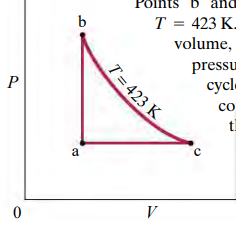
\includegraphics[width=0.3\textwidth]{figures/20-17.png}
\end{figure}
\newpage
\begin{center}
    \subsection*{\textbf{\textit{20-3 Carnot Engine}}}
\end{center}
\subsubsection*{
    8. What is the maximum efficiency of a heat engine whose
    operating temperatures are 550°C and 365°C?
}
\vspace{3.5in}
\subsubsection*{
    13. A nuclear power plant operates at 65\% of its maximum
    theoretical (Carnot) efficiency between temperatures of 660°C
    and 330°C. If the plant produces electric energy at the rate of
    1.2 GW, how much exhaust heat is discharged per hour?
}
\newpage
\subsubsection*{
    14. A Carnot engine performs work at the rate of 520 kW
    with an input of 950 kcal of heat per second. If the
    temperature of the heat source is 560°C, at what temperature
    is the waste heat exhausted?
}
\vspace{3.5in}
\subsubsection*{
    17. A heat engine utilizes a heat source at 580°C and has a
    Carnot efficiency of 32\%. To increase the efficiency to 38\%,
    what must be the temperature of the heat source?
}
\newpage
\begin{center}
    \subsection*{\textbf{\textit{20-5 and 20-6 Entropy}}}
\end{center}
\subsubsection*{
    33. A 7.5-kg box having an initial speed of 4.0$\frac m s$ slides
    along a rough table and comes to rest. Estimate the total
    change in entropy of the universe. Assume all objects are at
    room temperature (293 K).
}
\vspace{3.5in}
\subsubsection*{
    34. What is the change in entropy of 1.00 $m^3$ of water at 0°C
    when it is frozen to ice at 0°C?
}
\newpage
\subsubsection*{
    35. If 1.00 $m^3$ of water at 0°C is frozen and cooled to -10$\degree$C 
    by being in contact with a great deal of ice at -10$\degree$C,
    estimate the total change in entropy of the process.
}
\newpage
\begin{center}
    \subsection*{\textbf{\textit{General Problems}}}
\end{center}
\subsubsection*{
    77. The \textit{Stirling cycle}, shown in Fig. 20–27, is useful to describe
    external combustion engines as well as solar-power systems.
    Find the efficiency of the cycle in terms of the parameters
    shown, assuming a monatomic gas as the working substance. The
    processes \textit{ab} and \textit{cd} are isothermal whereas \textit{bd} and \textit{da} are at constant
    volume. How does it compare to the Carnot efficiency?
}
\begin{figure}[h]
    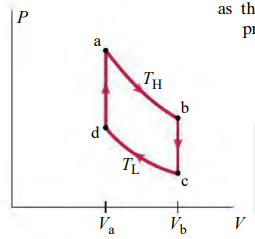
\includegraphics[width=0.3\textwidth]{figures/20-27.png}
\end{figure}

\newpage
\end{document}
